\documentclass[11pt,a4paper,titlepage,twocolumn]{ctexart}
\usepackage{mhchem,extarrows}
\usepackage{amsmath}
\usepackage{amsfonts}
\usepackage{amssymb}
\usepackage{graphicx}
\usepackage{hyperref}
\usepackage[left=2.54cm, right=2.54cm, top=3.18cm, bottom=3.18cm]{geometry}
\title{\textbf{{\huge 关于“测定空气中氧气的含量”实验的创新}}}
\author{青岛第二十六中学\quad 二〇一五级一班\\王愉扬}
\date{\today}
\begin{document}
	\maketitle
	\section{研究背景}
	
	在九年级上学期化学课本第7-1节中,介绍了测定空气中氧气的含量的方法,具体实验步骤如下:
	
\begin{center}
	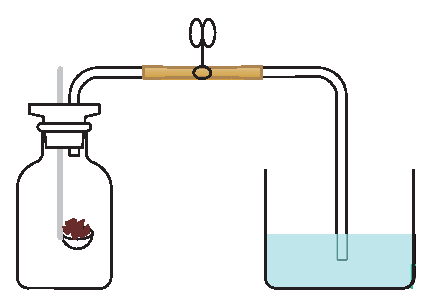
\includegraphics[width=0.8\linewidth]{fig/1}
\end{center}
	
	\begin{enumerate}
		\item 如图组装仪器,检查装置气密性。
		\item 在燃烧匙中装入过量红磷,置于酒精灯火焰上点燃后迅速放入集气瓶,塞紧瓶塞。
		\item 待燃烧完毕后容器恢复室温,打开止水夹,发现有一些水进入集气瓶内,且体积约占集气瓶体积的$\frac{1}{5}$。
		\item[·] 反应的化学方程式为:
		\[\ce{P4 + 5O2 \xlongequal{\mbox{\tiny 点燃}} 2P2O5}.\]
	\end{enumerate}

	由此,我们可以得出\textbf{“空气中氧气体积约占$\mathbf{\frac{1}{5}}$”}这一结论。但是经过理论分析和课堂实际操作,发现这一方法的缺点主要有二:
	
	\begin{itemize}
		\item 红磷的着火点过高,导致在瓶外点燃的时间过长,浪费时间。
		\item 在瓶外点燃可能会导致气体逸散,导致实验不准确,结果有误差。
	\end{itemize}
	
	\section{实验改进}
	\subsection{改进点燃不便和气体可能逸散的问题}
	\begin{itemize}
		\item 针对第一个问题,我们可以把红磷更换成白磷,经过查阅资料,我们发现白磷的着火点约在40℃左右,便于被点燃。
		\item 针对第二个问题,我们可以把容器密闭,用凸透镜或聚能激光笔产生的集中热量来点燃固体,示意图如下:\\
		\begin{center}
			
\includegraphics[width=0.4\linewidth]{fig/2}
		\end{center}
		
	\end{itemize}
	
	我们可以结合上述两种方案,设计出如下图所示的仪器:
	
	\begin{center}
		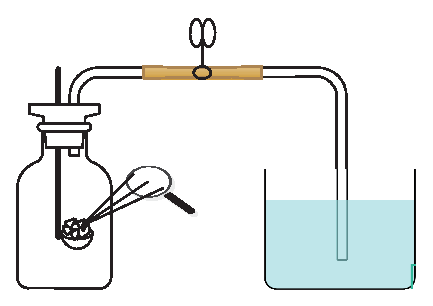
\includegraphics[width=0.8\linewidth]{fig/3}
	\end{center}
	

	经过测试,我们又发现这套装置还是有如下缺点:
	
	\begin{itemize}
		\item 点燃还是不够方便,若没有凸透镜或激光笔,还是要用酒精灯点燃。
		\item 水在集气瓶中,只能靠目测体积——刻度不够直观,不利于理解该结论。
	\end{itemize}
	
	\subsection{改进点燃不方便和体积不直观的问题}
	
	\begin{itemize}
		\item 针对第一个问题,我上网查资料得知,\textit{白磷的着火点约为40℃左右},所以我们可以直接把容器泡在开水中,这时,瓶内温度高于着火点,白磷就会自燃。
		\item 针对第二个问题,可以把水槽换成注射器,这样注射器减少的刻度就是消耗掉氧气的体积;再把集气瓶换成口径更细的试管,可以更加清晰地显示消耗氧气体积与总体积之比,示意图如下:\\
		\begin{center}
			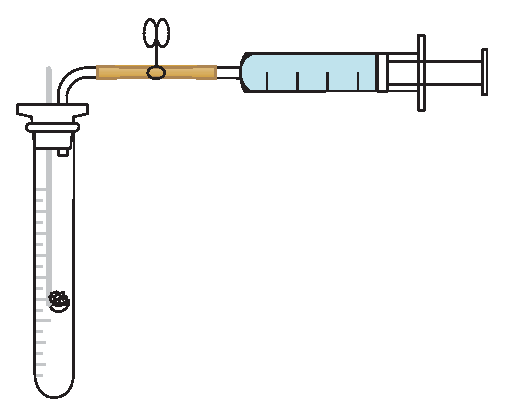
\includegraphics[width=0.8\linewidth]{fig/4}
		\end{center}
	\end{itemize}
		
	组合上述方案,又可以设计出如下图所示的仪器:
		
	\begin{center}
		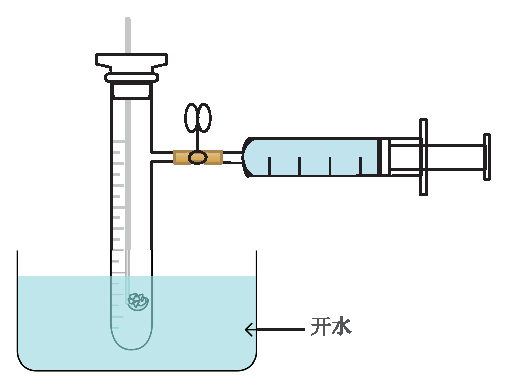
\includegraphics[width=0.8\linewidth]{fig/5}
	\end{center}
		
	经过试验,该套装置已能能较方便地点燃白磷,较好地反应体积的关系。但经过试验,仍发现了以下几个问题:
	
	\begin{itemize}
		\item 在试管中反应不太方便,特别是把燃烧匙伸入试管时容易撒漏。
		\item 注射器体积过小,装液量不够,不到集气瓶体积的$\frac{1}{5}$。
		\item 反应时放热,瓶内气压陡增,瓶塞容易弹开,需要在反应时用手按住。
	\end{itemize}
	
	经过尝试,我决定把试管恢复到集气瓶,在瓶塞上添加压强平衡注射器,并且把装有水的注射器换成量筒。
	
	但是反应后产生的五氧化二磷(\ce{P2O5})有毒,且剩余的白磷也属于有毒易燃危险品,这在课堂应用中是不能实施的,下一步要解决的问题是处理反应残余物。
	
	\subsection{改进生成物不环保的问题}
	
	经过网上查阅资料,我发现,\ce{P2O5}可以通过与水反应来消耗掉,反应的方程式为:
	\[\ce{P2O5 + 3H2O = 2H2PO4}.\]
	
	白磷可以与硫酸铜和水反应后生成无害物质,方程式为:
	{\footnotesize \[\ce{2P + 5CuSO4 + 8H2O = 5Cu + 2H3PO4 + 5H2SO4},\]}
	或:{\scriptsize \[\ce{11P + 15CuSO4 + 24H2O = 5Cu3P v + 6H3PO4 + 15H2SO4.}\]}
	
	在反应后的生成物中,\ce{H3PO4}、\ce{Cu3P}均无毒无害,不会污染环境。
	
	\section{改进结果}
	\subsection{实验器材}
	
	集气瓶、橡皮塞、注射器、止水夹、燃烧匙、导管若干
	
	\subsection{实验药品}
	
	加热至70℃的\ce{CuSO4}溶液、白磷
	
	\subsection{实验仪器}
	
	\begin{center}
		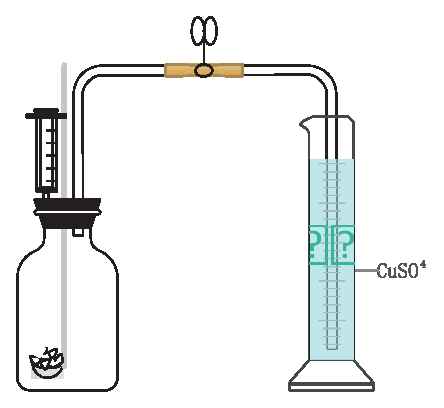
\includegraphics[width=0.6\linewidth]{fig/6}
	\end{center}
	
	\noindent\textbf{仪器说明:} \indent\par
	\begin{description}
		\item[注射器] 在反应时平衡集气瓶内气压,防止反应时白磷放热导致瓶内气压过大使瓶塞弹开。
		\item[量筒] 显示被吸入集气瓶\ce{CuSO4}的体积,刻度直观、准确。
		\item[\ce{CuSO4}] 反应前加热至高温后引燃白磷;反应后能够消耗有毒生成物。
	\end{description}
	
	\begin{enumerate}
		\item 如图,组装仪器。
		\item 检查装置气密性:打开止水夹,向上拉注射器活塞,使一部分高温\ce{CuSO4}进入集气瓶,若注射器显示的体积等于量筒内液体减少的体积,则装置气密性良好。这时记录量筒中液面的位置。
		\item 关闭止水夹,把注射器活塞推到``0''刻度处,等待白磷被热水引燃。
		\item 待白磷燃烧后,可以看到气压平衡注射器的活塞向上移动。燃烧完毕后,把集气瓶放入冷水中,使集气瓶内温度尽快恢复到室温。待气压平衡注射器的活塞恢复到``0''刻度后,打开止水夹,可以观察到有一些水被吸入集气瓶,并且量筒中液面下降。
		\item 待液体不再进入集气瓶内,记录量筒内液面高度。用反应前的高度减去反应后液面高度,即可得到被白磷消耗的氧气体积。
		\item 得出结论后,向上拉动注射器活塞,使更多\ce{CuSO4}进入集气瓶,没过燃烧匙。用力摇动集气瓶,使\ce{CuSO4}与白磷充分反应,完全消耗瓶内的残留物。
	\end{enumerate}
	
	\subsection{改进意义}
	
	\begin{enumerate}
		\item 改进了空气的逸散问题和燃烧物中白烟(\ce{P2O5})的污染。这样既能减少原来实验装置逸散空气的误差,也不污染环境,具有环保意识,防止空气污染。
		\item 注射器和量筒搭配巧妙。这一改进更加简化了读数环节,实验将清晰显示空气里\ce{O2}的体积。同时,注射器和量筒都有精密的刻度,能直接读出精确的数值,提高了实验的准确性。
		\item 注射器能在白磷燃烧时缓冲集气瓶内气压的骤然增大,从而能防止冲塞现象的发生,起到了较好的缓冲作用
		\item 在引燃燃烧物\textit{(白磷)}方面设计巧妙。实验不仅方便操作,还环保,让实验现象更加容易观察。
		\item \textbf{总之,通过创新性地开展实验设计,在实验装置方面做了一些有益的改进,让实验更加精确,操作性更强;同时我在实验中也培养了实验探索、创新精神,发展了创新思维。}
	\end{enumerate}
	
\end{document}